\documentclass[a4paper,12pt]{article}
\usepackage[utf8]{inputenc}
\usepackage[french]{babel}
\usepackage[T1]{fontenc}
\usepackage[top=2cm,bottom=2cm,left=2cm,right=2cm]{geometry}
\usepackage{graphicx}
\usepackage{wrapfig}
\usepackage{url}

\begin{document}

\begin{titlepage}
	\begin{center}
		\Large{Année universitaire 2016-2017}\\
		\Large{Université de Caen Basse-Normandie}\\[1cm]
		
		\huge{Rapport sur la mise en place du parse XML avec Python afin d'utiliser un fichier de configuration XML}\\
		\vspace{3cm}
		
		Alexis Carreau
		
	\normalsize{\textit{ ~ L2 Informatique}}\\
		\medskip
		\vspace{2cm}
		
	\begin{figure}[h!]
			\begin{center}
				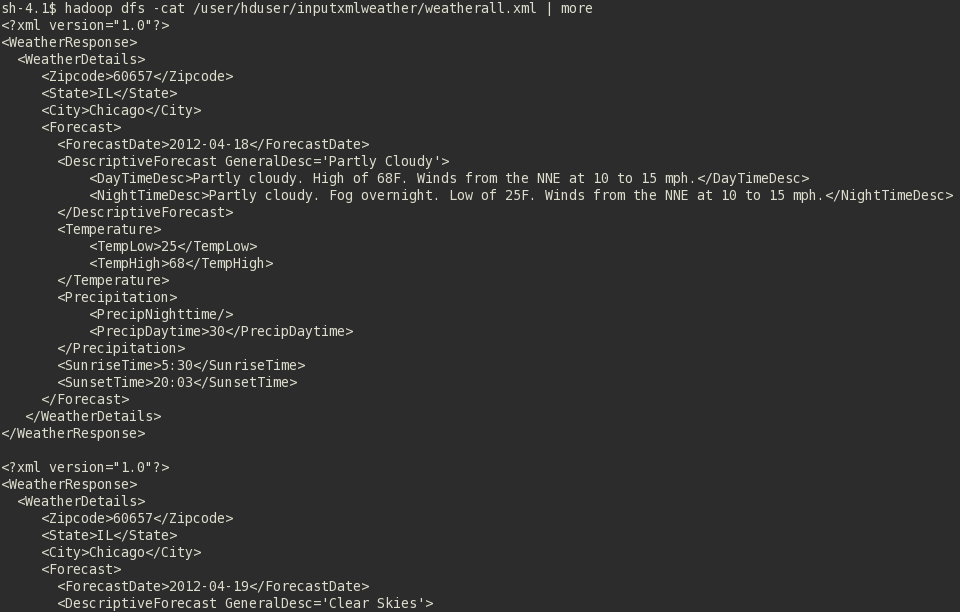
\includegraphics[scale=0.7]{images/intro.png}
				\caption{Exemple de fichier XML}
			\end{center}
		\end{figure}
				
	\end{center}
\end{titlepage}

\tableofcontents
\newpage

\section{La nécessité du XML}

Au fur et à mesure de l'ajout de fonctionnalités dans notre IDE, l'utilisation du XML s'est imposée du fait de son efficacité et également par convention. Nous devions ainsi lire, parcourir et écrire dans un fichier XML.
	
\section{XML et Python : LXML}

Pour ce faire, nous avons utilisé LXML, qui nous permet d'utiliser des outils de parse XML dans notre IDE avec Python. En effet, l'outil "etree", après son import, nous permet de parser un fichier XML et de le parcourir et modifier par la suite.
		
Nous avons beaucoup d'outils disponibles pour parcourir et modifier un fichier XML : 

\begin{figure}[h!]
			\begin{center}
				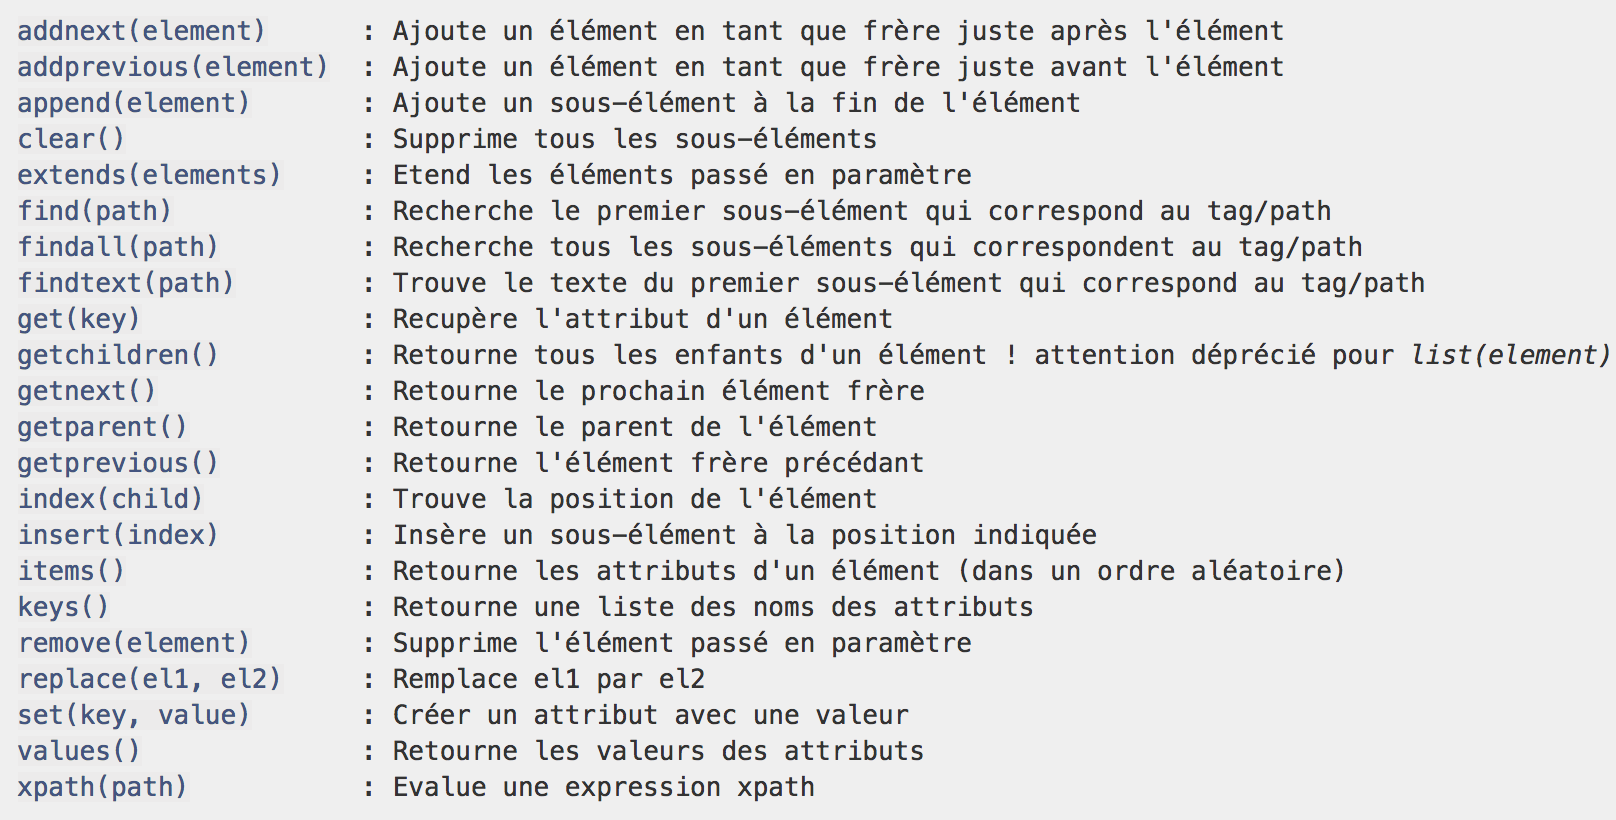
\includegraphics[scale=0.6]{images/lxml.png}
				\caption{Outils LXML disponibles}
			\end{center}
		\end{figure}

Nous avions donc ainsi tous les outils nécessaires pour utiliser le XML dans notre IDE. Nous avons d'ailleurs utilisé les outils "find", "getchildren" et "xpath" pour le parcours du fichier XML.

\section{Le module XML et le fichier de configuration}

Nous avons donc ainsi créer un module XML pour les fonctions de parcours et d'écriture de fichier XML et bien entendu, le fichier de configuration XML. Voici d'ailleurs leur disposition dans notre IDE, ils sont à la racine du projet:

\newpage

\begin{figure}[h!]
			\begin{center}
				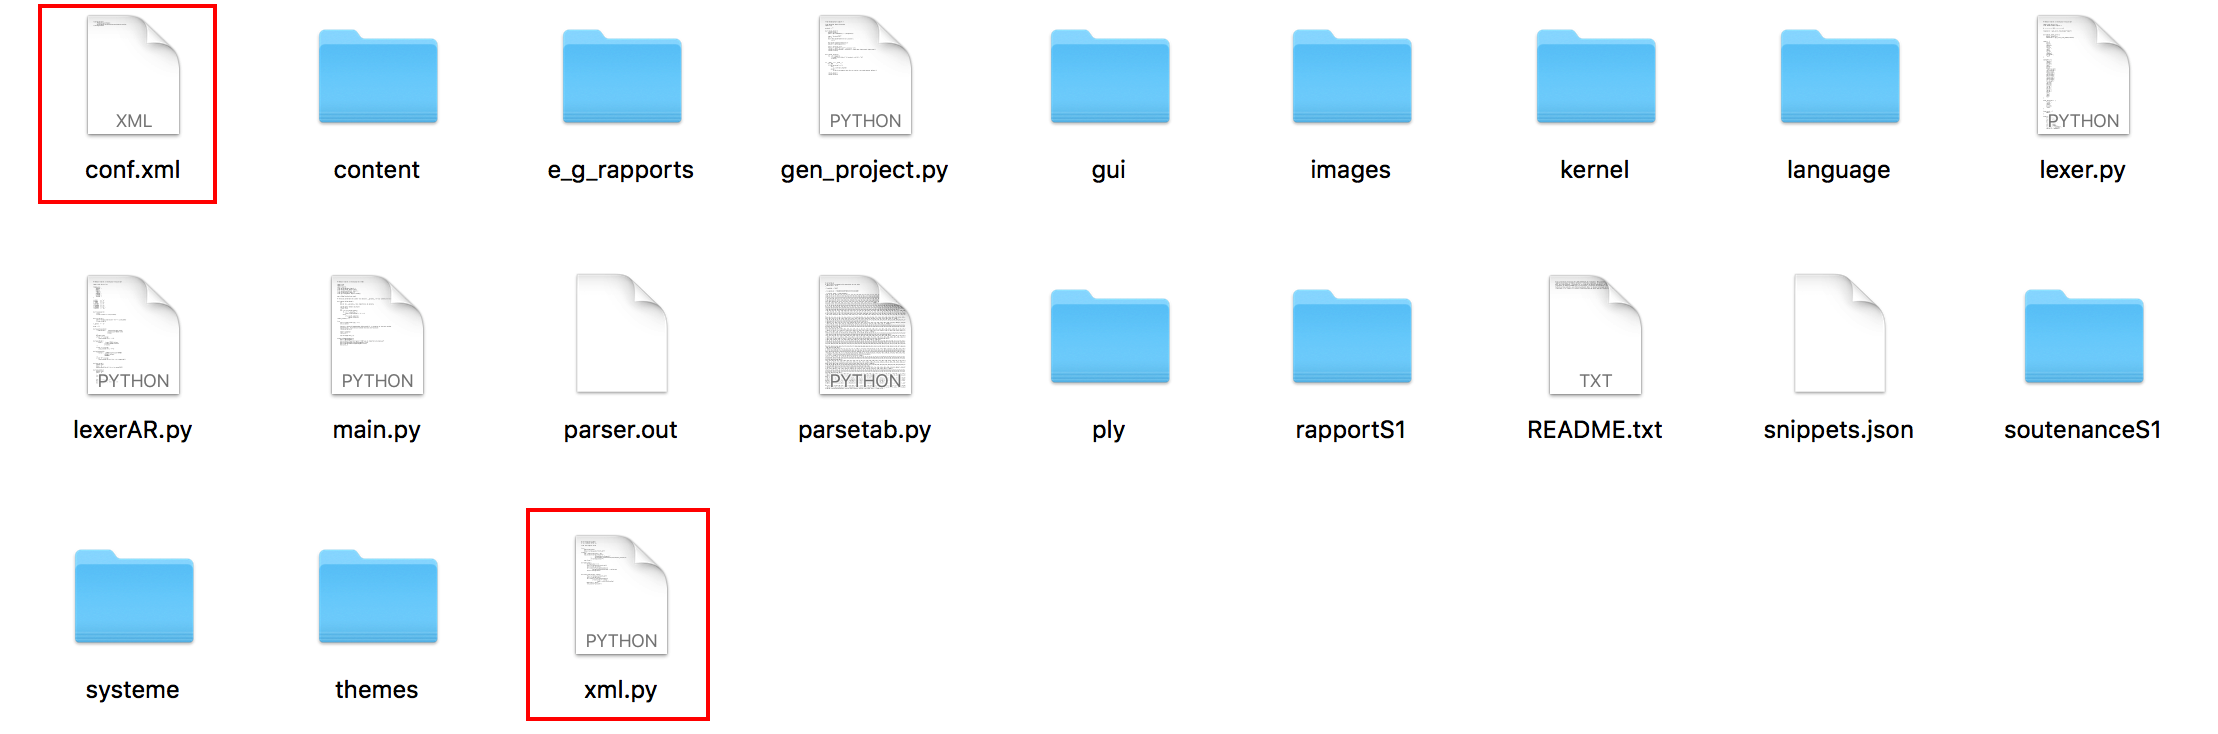
\includegraphics[scale=0.23]{images/dossier.png}
				\caption{Disposition du module et du fichier de configuration}
			\end{center}
		\end{figure}
		
Dans le module XML, nous avons une fonction open\_xml, qui ouvre, parse et parcours le fichier de configuration XML pour retourner un dictionnaire avec comme clés le nom des balises XML, et comme valeurs la valeur des balises. Nous avons également une fonction write\_xml qui permet d'écrire des modifications dans le fichier de configuration. On rentre le nom d'une balise et la valeur voulue en arguments, la fonction trouve la balise et lui associe cette valeur, puis nous écrivons dans le fichier. Enfin, pour éviter tout problème, si le fichier de configuration n'existe pas, on le créé et lui ajoute les valeurs de configuration de base. 
		
Dans le fichier de configuration XML, nous utilisons une balise pour stocker, le thème sélectionné actuellement, ainsi que le booléen True / False suivant l'activation ou non de l'assistance vocale dans l'interface graphique.
		
\begin{figure}[h!]
			\begin{center}
				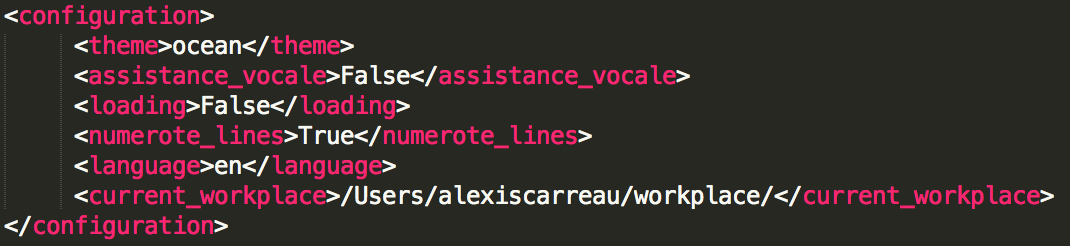
\includegraphics[scale=0.6]{images/conf.png}
				\caption{Fichier de configuration}
			\end{center}
		\end{figure}

\section{L'application dans notre IDE}

Après avoir défini les différentes fonctions et stockage de variables nécessaires, il ne restait plus qu'à implémenter le XML dans notre IDE. Nous l'avons pour le moment implémentés pour les thèmes et l'assistance vocale.

\subsection{Les thèmes}

Pour implémenter le XML pour les thèmes nous devions donc adapter les différentes fonctions déjà définies. Nous l'avons donc fait dans le module themes.

Grâce au dictionnaire, nous pouvons ainsi récupérer la valeur du thème actuel en écrivant configuration['theme']. Pour modifier le thème, nous utilisons la fonction write\_xml afin d'associer la valeur en argument à la valeur de la balise theme dans le fichier XML. 

Nous pouvons voir que la mise à jour du fichier XML s'effectue bien suivant le thème sélectionné du fait de sa mémorisation à l'ouverture et fermeture de l'IDE, voilà l'interface graphique de la sélection du thème : 

\begin{figure}[h!]
			\begin{center}
				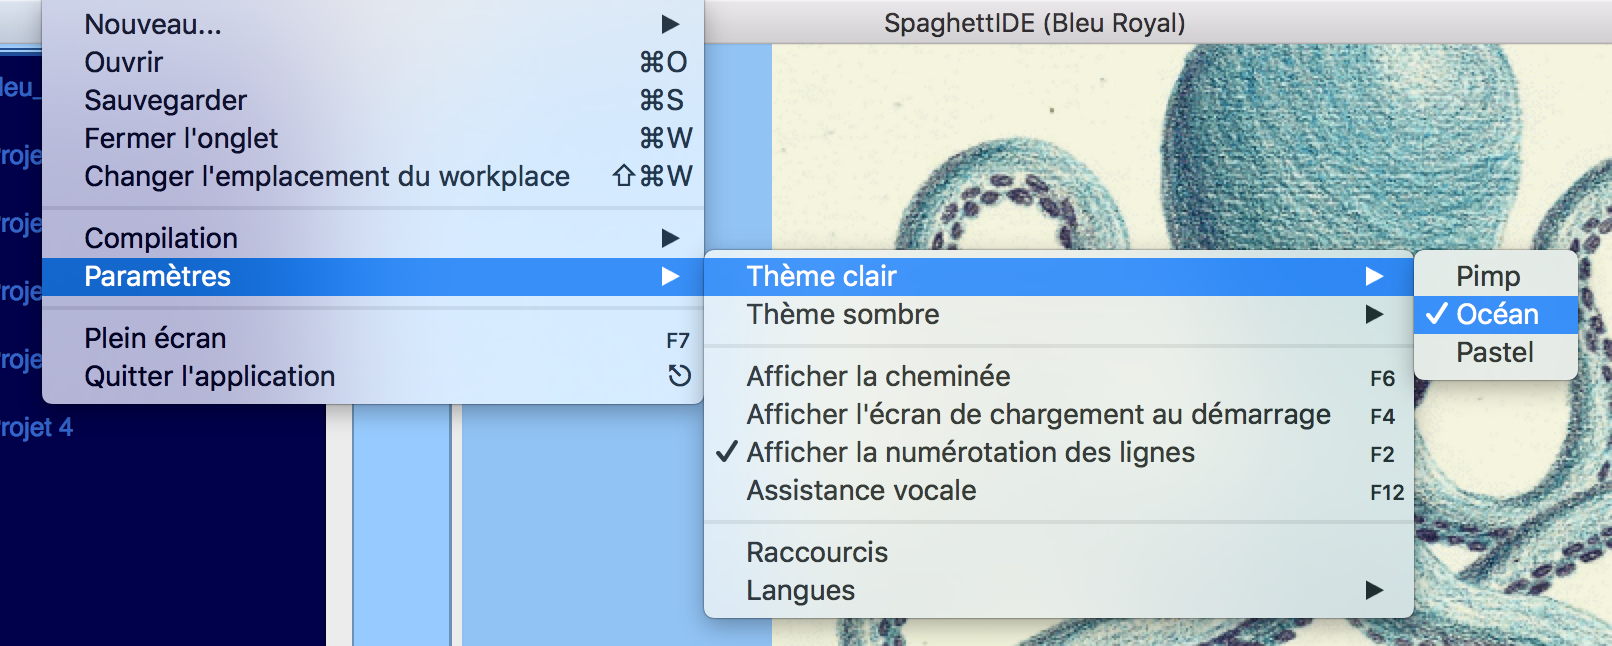
\includegraphics[scale=0.6]{images/themes_selection.png}
				\caption{Interface graphique de la sélection du thème}
			\end{center}
		\end{figure}

\subsection{L'assistance vocale}

Pour implémenter le XML pour l'assistance vocale nous devions donc encore une fois adapter les différentes fonctions déjà définies. Nous l'avons donc d'abord fait dans le module GUI. 

Grâce au dictionnaire, nous pouvons ainsi récupérer la valeur de l'activation de l'assistance vocale actuelle en écrivant configuration['assistance\_vocale']. Nous pouvons ainsi faire des conditions. Nous utilisons encore une fois la fonction write\_xml afin d'associer la valeur en argument à la valeur de la balise assistance\_vocale dans le fichier XML. 

Nous avons adapté les différentes fonctions déjà définies dans le module MENU. Avec encore une fois des conditions, nous avons fait en sorte que si l'assistance vocale était désactivée alors elle n'est pas cochée dans le menu fichier et inversement.

Nous pouvons voir que la mise à jour du fichier XML s'effectue bien suivant l'activation ou la désactivation de l'assistance vocale du fait de sa mémorisation à l'ouverture et fermeture de l'IDE, voilà l'interface graphique de la sélection de l'assistance vocale : 

\begin{figure}[h!]
			\begin{center}
				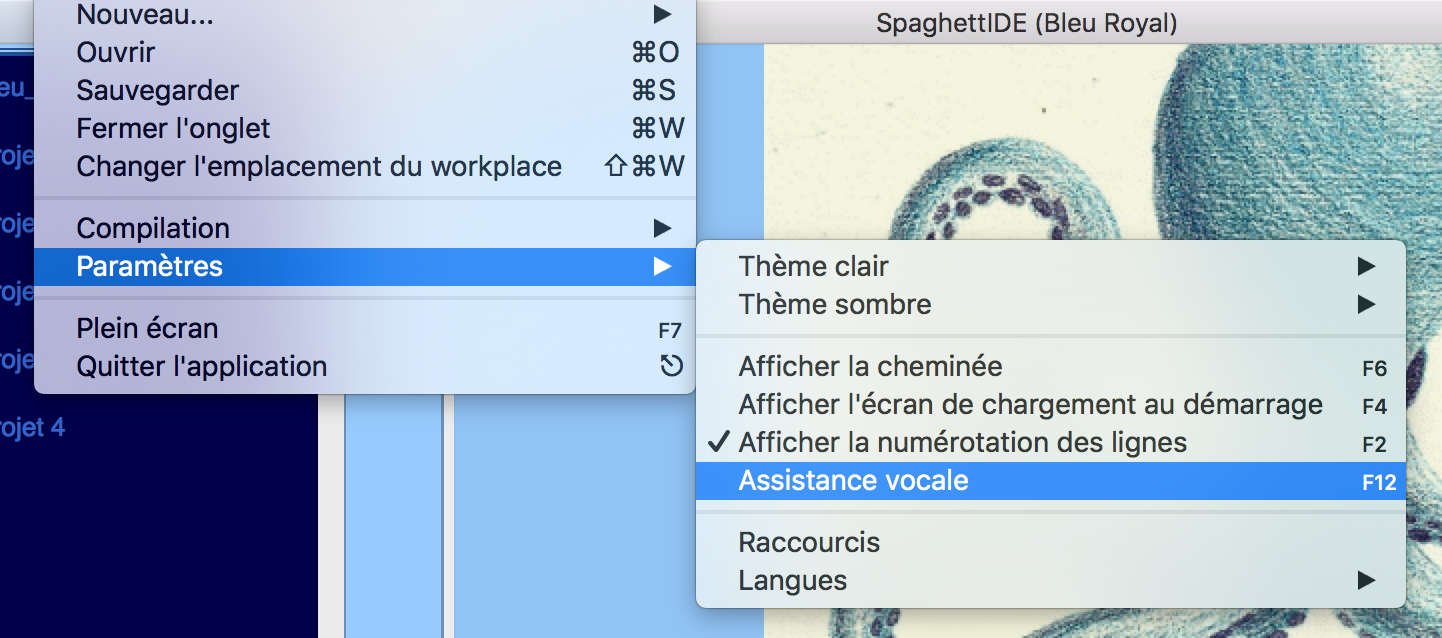
\includegraphics[scale=0.5]{images/assistance_vocale.png}
				\caption{Interface graphique de la sélection de l'assistance vocale}
			\end{center}
		\end{figure}
		
\section{Conclusion}

En conclusion, nous pouvons dire que le XML est vraiment très pratique et nous comptons l'utiliser dans d'autres cas pour notre IDE, par exemple, dès que l'on aura d'autres configurations à ajouter, donc dans le fichier de configuration. Il est prévu d'y ajouter tous les noms des thèmes en plus de celui sélectionné afin d'améliorer le code, notamment son aspect visuel.
		
\end{document}